\newpage
\section{Ensembles et mesures}


%\begin{tikzpicture}
    %\draw (-3,-2) rectangle (3,2);
    %\node at (-2.7,1.7) {$\Omega$};
    % \draw (-1,0) ellipse [x radius=2.5, y radius=1.5] node[left] {$\Omega$};
%\end{tikzpicture}
\begin{tcolorbox}[breakable,colback=white!100, colframe=cyan!70!blue, title=Vocabulaire des ensembles]
\noindent
\begin{minipage}{0.3\textwidth}
    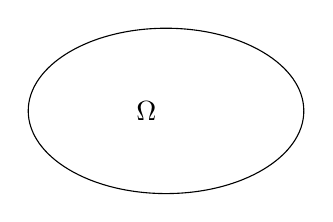
\begin{tikzpicture}[scale=0.7]
        \draw (-1,0) ellipse [x radius=2.5, y radius=1.5] node[left] {$\Omega$};
    \end{tikzpicture}
\end{minipage}%
\hfill
\begin{minipage}{0.7\textwidth}
    Un \textbf{ensemble} $\Omega$.\\
    \ex{ \begin{eleve}$\Omega =$ les élèves de la classe.\end{eleve}}
\end{minipage}
\vspace{0.5cm}
\hrule
\vspace{0.5cm}
\noindent
\begin{minipage}{0.3\textwidth}
    \center
$ \emptyset $
\end{minipage}%
\hfill
\begin{minipage}{0.7\textwidth}
    L'\textbf{ensemble vide} $ \emptyset $.
     \ex{.}
\end{minipage}
\vspace{0.5cm}
\hrule
\vspace{0.5cm}
\noindent
\begin{minipage}{0.3\textwidth}
    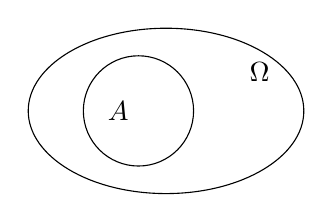
\begin{tikzpicture}[scale=0.7]
        \draw (-1,0) ellipse [x radius=1, y radius=1] node[left] {$A$};
        \draw (-0.5,0) ellipse [x radius=2.5, y radius=1.5];
        \node at (1.2,0.7) {$\Omega$};
    \end{tikzpicture}
\end{minipage}%
\hfill
\begin{minipage}{0.7\textwidth}
    $A \subset \Omega$. $A$ est \textbf{inclus} dans $\Omega$, $A$ est un \textbf{sous-ensemble} de $\Omega$.\\
    \ex{\begin{eleve}$\Omega =$ les élèves de la classe.\\ 
    $A =$ les élèves de la classe ayant leur anniversaire en juillet. \end{eleve}}
\end{minipage}
\vspace{0.5cm}
\hrule
\vspace{0.5cm}
\noindent
\begin{minipage}{0.3\textwidth}
    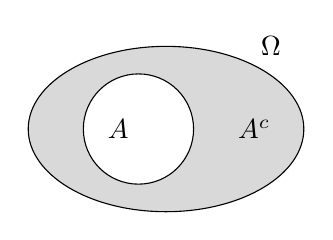
\begin{tikzpicture}[scale=0.7]
        \fill[gray!30] (-0.5,0) ellipse [x radius=2.5, y radius=1.5];
        \fill[white] (-1,0) ellipse [x radius=1, y radius=1];
        \draw (-1,0) ellipse [x radius=1, y radius=1] node[left] {$A$};
        \draw (-0.5,0) ellipse [x radius=2.5, y radius=1.5];
        \node at (1.4,1.5) {$\Omega$};
        \node at (1.1,0) {$A^c$};
    \end{tikzpicture}
\end{minipage}%
\hfill
\begin{minipage}{0.7\textwidth}
    $A^c$, l'ensemble \textbf{complémentaire} de $A$ dans $\Omega$.\\
    \ex{\begin{eleve}$\Omega =$ les élèves de la classe.\\
    $A =$ les élèves de la classe ayant leur anniversaire en juillet.\\
    $A^c =$ les élèves de la classe n'ayant pas leur anniversaire en juillet.\\\end{eleve}}
\end{minipage}
\vspace{0.5cm}
\hrule
\vspace{0.5cm}
\noindent
\begin{minipage}{0.3\textwidth}
    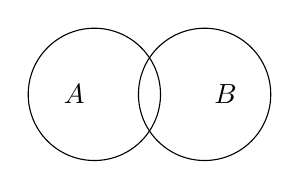
\begin{tikzpicture}[scale=0.7]
        % Shade A and B fully
        %\fill[gray!30] (-1,0) circle (1.2);
        %\fill[gray!30] (1,0) circle (1.2);

        % Draw sets
        \draw (-1,0) circle (1.2) node[left] {$A$};
        \draw (1,0) circle (1.2) node[right] {$B$};
    \end{tikzpicture}
\end{minipage}%
\hfill
\begin{minipage}{0.7\textwidth}
   Deux ensembles ayant une intersection.\\
   \ex{\begin{eleve}
   $A = $ les mammifères\\
   $B = $ les animaux vivants dans l'eau.\end{eleve}}
\end{minipage}
\vspace{0.5cm}
\hrule
\vspace{0.5cm}
\noindent
\begin{minipage}{0.3\textwidth}
    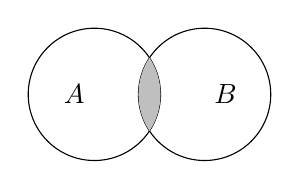
\begin{tikzpicture}[scale=0.7]
        \draw (-1,0) circle (1.2) node[left] {$A$};
        \draw (1,0) circle (1.2) node[right] {$B$};
        \begin{scope}
            \clip (-1,0) circle (1.2);
            \fill[gray!50] (1,0) circle (1.2);
        \end{scope}
    \end{tikzpicture}
\end{minipage}%
\hfill
\begin{minipage}{0.7\textwidth}
    L'\textbf{intersection} $A \cap B$.\\
    \ex{\begin{eleve}
   $A = $ les mammifères\\
   $B = $ les animaux vivants dans l'eau.\\
   $A \cap B = $ les mammifères vivants dans l'eau (le dauphin, la baleine, l'ornithorynque...)\\


    $\Omega =$ les élèves de la classe.\\
    $A =$ les élèves de la classe ayant leur anniversaire en juillet.\\
   $A \cap \Omega = A$ les élèves de la classe ayant leur anniversaire en juillet.\end{eleve}}
\end{minipage}
\vspace{0.5cm}
\hrule
\vspace{0.5cm}
\noindent
\begin{minipage}{0.3\textwidth}
    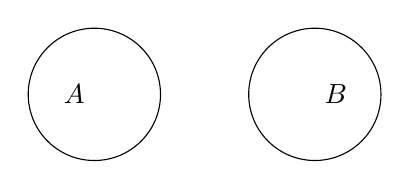
\begin{tikzpicture}[scale=0.7]
        \draw (-2,0) circle (1.2) node[left] {$A$};
        \draw (2,0) circle (1.2) node[right] {$B$};
    \end{tikzpicture}
\end{minipage}%
\hfill
\begin{minipage}{0.7\textwidth}
   Deux ensembles \textbf{disjoints} $A$ et $B$. L'intersection est vide. $A \cap B = \emptyset$.\\
   \ex{\begin{eleve}
   $A =$ Les personnes nées en juillet.\\
   $B =$ Les personnes nées en mars.\end{eleve}}
\end{minipage}
\vspace{0.5cm}
\hrule
\vspace{0.5cm}
\noindent
\begin{minipage}{0.3\textwidth}
    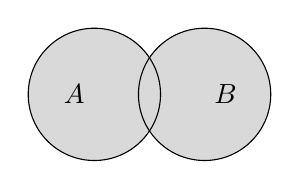
\begin{tikzpicture}[scale=0.7]
        % Shade A and B fully
        \fill[gray!30] (-1,0) circle (1.2);
        \fill[gray!30] (1,0) circle (1.2);

        % Draw sets
        \draw (-1,0) circle (1.2) node[left] {$A$};
        \draw (1,0) circle (1.2) node[right] {$B$};
    \end{tikzpicture}
\end{minipage}%
\hfill
\begin{minipage}{0.7\textwidth}
    $A \cup B$. L'\textbf{union} des ensembles $A$ et $B$.\\
    \ex{\begin{eleve}
    $A =$ Les personnes nées en juillet.\\
   $B =$ Les personnes nées en mars.\\
   $A \cup B = $ Les personnes nées en juillet ou en mars.\end{eleve}}
\end{minipage}
\vspace{0.5cm}
\hrule
\vspace{0.5cm}
\noindent
\begin{minipage}{0.3\textwidth}
    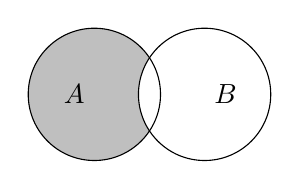
\begin{tikzpicture}[scale=0.7]
        \begin{scope}
            \clip (-1,0) circle (1.2);
            \fill[gray!50] (-3,-2) rectangle (3,2);
            \begin{scope}
                \clip (1,0) circle (1.2);
                \fill[white] (-3,-2) rectangle (3,2);
            \end{scope}
        \end{scope}
        \draw (-1,0) circle (1.2) node[left] {$A$};
        \draw (1,0) circle (1.2) node[right] {$B$};
    \end{tikzpicture}
\end{minipage}%
\hfill
\begin{minipage}{0.7\textwidth}
$A \setminus B$. $A$ \textbf{sans} $B$.\\
\ex{\begin{eleve}
$A =$ les élèves nées en juillet.\\
$B =$ les élèves portant des lunettes.\\
$A \setminus B =$ les élèves nées en juillet ne portant pas de lunettes.\end{eleve}}
\end{minipage}
\end{tcolorbox}
\vspace{1cm}

\newpage
On peut alors vouloir "mesurer" certains ensembles, selon ce qu’on cherche à quantifier.
Pour cela, il faut d’abord décider sur quels ensembles on peut mesurer quelque chose et définir une règle de mesure cohérente.

\ex{.\\
\begin{enumerate}
    \item $\Omega =$ les élèves de la classe. $A =$ les élèves de la classe ayant leur anniversaire en juillet.\\ Une mesure : \begin{eleve}nombre d'élèves.\end{eleve}
    \item $\Omega =$ l'école Christ-Roi. $A =$ la salle de gym.\\ Une mesure : \begin{eleve}surface en mètres carrés.\end{eleve}\\ Une autre mesure : \begin{eleve}capacité maximale en nombre de personnes.\end{eleve}
    \item $\Omega =$ tous les aliments de mon sac de courses. $A =$ les pommes dans mon sac.\\ Une mesure : \begin{eleve}masse en kg.\end{eleve}\\ 
    Une autre mesure : \begin{eleve}prix en euros.\end{eleve}\\ Une autre mesure : \begin{eleve}nombre d'objets.\end{eleve}
    \item $\Omega =$ le couloir à côté de la classe. $A = $ une partie du couloir.\\ 
    Une mesure : \begin{eleve}longueur en mètres.\end{eleve}
    \item $\Omega =$ la journée. $A =$ la pause de midi.\\ 
    Une mesure : \begin{eleve}temps en heures.\end{eleve} \\ 
    Une autre mesure : \begin{eleve}proportion de la journée.\end{eleve}
\end{enumerate}
}

Il y a plusieurs conditions pour qu'un ensemble soit mesurable. Nous n'irons pas dans les détails dans ce chapitre. Nous ne travaillerons qu'avec des espaces mesurables dans la suite du chapitre.\\

\newpage
On peut alors définir la mesure.
\begin{tcolorbox}[colback=cyan!5, colframe=cyan!70!blue, title=Définition d'une mesure]
\defn{Une \textbf{mesure} $\mu$ sur un ensemble $\Omega$ est une fonction qui associe à chaque ensemble mesurable $A \subset \Omega$ un nombre réel $\mu(A)$, qui respecte les 3 propriétés suivantes :}\label{def:mesure}

\begin{enumerate}
    \item $\mu(\emptyset) = 0$.
    \item \textbf{Positivité} : $\mu(A) \ge 0$.
    \item \textbf{Additivité dénombrable} : si $(A_n)_{n \ge 1}$ est une suite d’ensembles disjoints deux à deux, alors
        \[
        \mu(A_1 \cup A_2 \cup A_3 \cup \dots) = \mu(A_1) + \mu(A_2) + \mu(A_3) + \dots
    \]
    Cela signifie que la mesure de l’union d’ensembles disjoints est égale à la somme des mesures de chacun.

    
    \[
        \mu\Big(\bigcup_{n=1}^{\infty} A_n\Big) = \sum_{n=1}^{\infty} \mu(A_n).
    \]
En particulier, si $A\in \Omega$ et $B \in \Omega $ sont disjoints,
\[
\mu(A \cup B) = \mu(A) + \mu(B)
\]
\end{enumerate}
\end{tcolorbox}

\begin{figure}[H]
    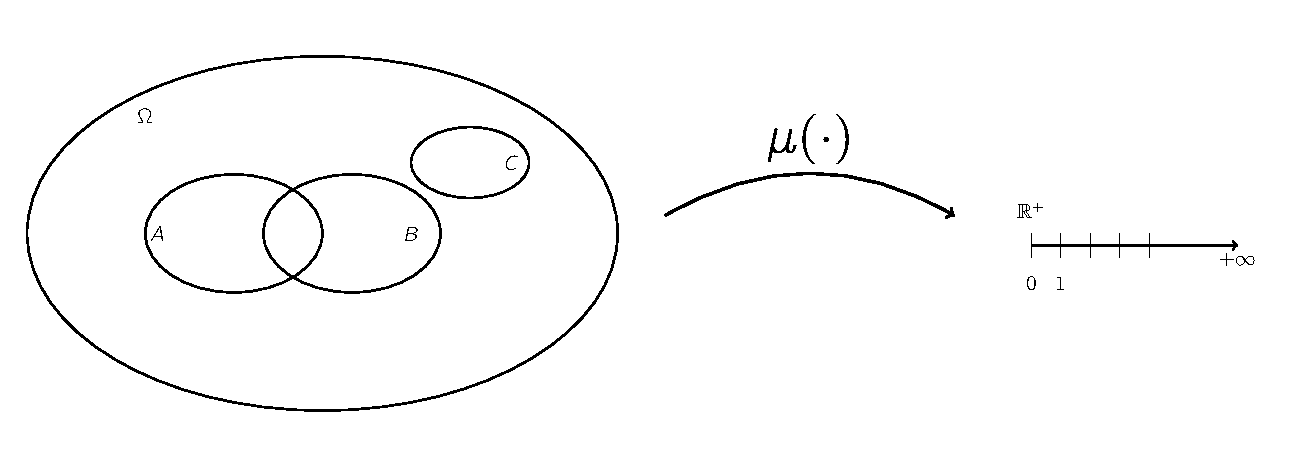
\includegraphics[scale = 0.7]{./tikz_standalone/measure_1.pdf}
\end{figure}
   \ex{
   $\Omega =$ Les élèves de la classe.\\
   On définit la mesure $\mu$ comme le nombre d'élèves dans l'ensemble.\\
   $A =$ Les élèves ayant leur anniversaire en juillet, $\qquad \mu(A) = $\\
   $B =$ Les élèves ayant leur anniversaire en mars, $\qquad \mu(B) = $\\
   Les deux ensembles $A$ et $B$ sont disjoints ($A \cap B = \emptyset$ : personne ne peut être né en même temps en mars et en juillet).\\
    $A \cup B =$ Les élèves nés en juillet ou en mars, $\qquad \mu(A \cup B) =$}

\newpage
    \begin{tcolorbox}[colback=magenta!5, colframe=red!50!blue, title=Propriétés des ensembles complémentaires]
    \prop{Si $A\in\Omega$, et $A^c = \Omega \setminus A $ le complémentaire de $A$ dans $\Omega$. \\Par définition, $A$ et $A^c$ sont disjoints et $A\cup A^c= \Omega$ donc $$\mu (A) + \mu(A^c)= \mu(\Omega)$$}
    \end{tcolorbox}
      \ex{
   $\Omega =$ Les élèves de la classe. $\qquad \mu(\Omega) = $\\
   Avec la mesure $\mu$ étant le nombre d'élèves dans l'ensemble.\\
   $A =$ Les élèves ayant leur anniversaire en juillet, $\qquad \mu(A) = $\\
   $A^C =$ Les élèves n'ayant pas leur anniversaire en juillet, $\qquad \mu(A^c) = $\\
   $\mu (A) + \mu(A^c)= $}

\begin{tcolorbox}[colback=magenta!5, colframe=red!50!blue, title=Propriétés de l'union des ensembles quelconques]
    \prop{Si $A\in\Omega$, et $B \in \Omega$ des ensembles quelconques, alors $$ \mu (A\cup B) = \mu(A) + \mu(B) - \mu(A\cap B)$$}
\end{tcolorbox}
    \ex{
   $\Omega =$ Les élèves de la classe.\\
   Avec la mesure $\mu$ étant le nombre d'élèves dans l'ensemble.\\
   $A =$ Les élèves portant un jeans, $\qquad \mu(A) = $\\
   $B =$ Les élèves portant des lunettes, $\qquad \mu(B) = $\\
   $A \cup B =$ Les élèves portant un jeans ou des lunettes, $\qquad \mu (A) + \mu(B)= $}

   \vspace{0.5cm}
   \begin{minipage}{0.3\textwidth}
    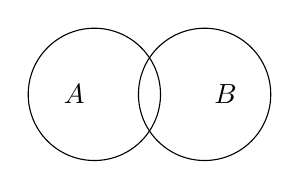
\begin{tikzpicture}[scale=0.7]
        % Shade A and B fully
        %\fill[gray!30] (-1,0) circle (1.2);
        %\fill[gray!30] (1,0) circle (1.2);

        % Draw sets
        \draw (-1,0) circle (1.2) node[left] {$A$};
        \draw (1,0) circle (1.2) node[right] {$B$};
    \end{tikzpicture}
\end{minipage}%